\begin{frame}
  \frametitle{Affine representations}

  \begin{itemize}
  \item Not possible to express the Navier-Stokes problem as finite sums
    \[
      \bm A_h(\bm \mu) = \textstyle \sum_i \xi_i(\bm \mu) \bm A_i, \qquad
      \bm f_h(\bm \mu) = \textstyle \sum_i \chi_i(\bm \mu) \bm f_i
    \]
  \item Instead, we use truncated polynomial series in $\varphi$.\footcite{Fonn2018fdc}
  \item We can expect about $10$ digits of accuracy with a reasonable number of terms
    (${\sim}25$ for TH, ${\sim}75$ for DC).
  \item Recall: the intention is to encode \emph{all} parameters explicitly in the representation of
    the bi- or trilinear forms.
  \end{itemize}
\end{frame}

\begin{frame}
  \frametitle{Affine representations (cont.)}

  \begin{itemize}
  \item The Jacobian of the domain transformation can be expressed as
    \[
      \bm J = \bm R(a) (\bm I + \varphi \bm P \bm Q)
    \]
  \item $\bm R$ is a rotation matrix through angle $a$.
  \item $a(r) = \varphi \theta(r)$, where $\theta$ is any suitably smooth
    ``canonical'' angle function
    \begin{center}
      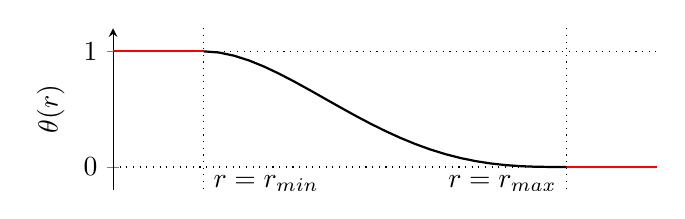
\begin{tikzpicture}
        \begin{axis}[
          ylabel={$\theta(r)$},
          width=0.7\textwidth,
          height=0.3\textwidth,
          axis lines=left,
          hide x axis,
          ymin=-0.2, ymax=1.2,
          ytick={0,1},
          yticklabels={$0$,$1$},
          ]
          \addplot[thick, red, domain=0:1] {1};
          \addplot[thick, red, domain=5:6] {0};
          \addplot[thick, domain=1:5] {(1-((x-1)/4))^3 * (3*(x-1)/4+1)};
          \draw[dotted] (axis cs:1,1.2) -- (axis cs:1,-0.2);
          \draw[dotted] (axis cs:5,1.2) -- (axis cs:5,-0.2);
          \draw[dotted] (axis cs:0,0) -- (axis cs:5,0);
          \draw[dotted] (axis cs:1,1) -- (axis cs:6,1);
          \node[anchor=south west] at (axis cs:1,-0.30) {$r=r_\text{min}$};
          \node[anchor=south east] at (axis cs:5,-0.30) {$r=r_\text{max}$};
        \end{axis}
      \end{tikzpicture}
    \end{center}
  \item $\bm Q = \frac{\theta'}{r} \hat{\bm r} \hat{\bm r}^\intercal$,
    and $\bm P = \bm R(\pi/2)$.
  \end{itemize}
\end{frame}

\begin{frame}
  \frametitle{Affine representations (cont.)}

  \begin{itemize}
  \item It can also be determined that, as expected, $\det \bm J = 1$.
  \item And
    \[
      \bm J^{-1} = \left( \bm I - \varphi \bm P \bm Q \right)
      \bm R(a)^\intercal.
    \]
  \item As for $\bm R$, we have
    \[
      \bm R(a) = \sum_i \frac{a^i}{i!} \bm P^i = \sum_i \varphi^i \bm R_i
    \]
    where $\bm R_i = \theta^i \bm P^i / i!$
  \item Summary: any expression involving $\bm J$, $\det \bm J$ and
    $\bm J^{-1}$ can be given an affine representation in terms of a
    truncated series expansion of $\bm R$.
  \end{itemize}
\end{frame}

\begin{frame}
  \frametitle{Affine representations (TH)}

  \begin{align*}
  ({\bm\pi}^*_{\bm\mu}a)(
    \hat{\bm u},
    \hat{\bm w};
    \varphi
  )
  &= \nu \int_{\hat{\Omega}} (\bm J^{-\intercal} \nabla) \hat{\bm u} : (\bm J^{-\intercal} \nabla)
    \hat{\bm w} |\bm J| \\
  &= \nu \int_{\hat{\Omega}} \nabla \hat{\bm u} : (\bm J^{-1} \bm J^{-\intercal} \nabla) \hat{\bm w}
    |\bm J|,
  \end{align*}
  and we find (based on the above) that
  \begin{align*}
    \bm J^{-1} \bm J^{-\intercal}
    &= (\bm I - \varphi \bm P \bm Q) \bm R^\intercal
      \bm R (\bm I + \varphi \bm Q \bm P) \\
    &= \bm I + \varphi \underbrace{(\bm Q \bm P - \bm P \bm Q)}_{\bm D_1}
      - \varphi^2 \underbrace{\bm P \bm Q^2 \bm P}_{\bm D_2} \\
    &= \bm I + \varphi \bm D_1 - \varphi^2 \bm D_2.
  \end{align*}
\end{frame}

\begin{frame}
  \frametitle{Affine representations (TH; cont.)}

  Thus we have, in three terms
  \begin{align*}
    ({\bm\pi}^*_{\bm\mu}a)(
    \hat{\bm u},
    \hat{\bm w};
    \varphi
    ) &=
    \nu \int_{\hat{\Omega}} \nabla \hat{\bm u} : \nabla \hat{\bm w} \\
    &+ \nu \varphi \int_{\hat{\Omega}}
    \nabla \hat{\bm u} : (\bm D_1 \nabla) \hat{\bm w} \\
    &- \nu \varphi^2 \int_{\hat{\Omega}}
    \nabla \hat{\bm u} : (\bm D_2 \nabla) \hat{\bm w}.
  \end{align*}
\end{frame}

\begin{frame}
  \frametitle{Affine representations (TH; cont.)}

  Similarly,
  \begin{align*}
    ({\bm\pi}^*_{\bm\mu}b)(
    \hat{p},
    \hat{\bm w};
    \varphi
    ) =
    \int_{\hat{\Omega}} \hat{p} (\bm J^{-\intercal} \nabla) \cdot \hat{\bm w} |\bm J|
    = \int_{\hat{\Omega}} \hat{p} \bm J^{-\intercal} : \nabla \hat{\bm w} |\bm J|,
  \end{align*}
  and we have
  \begin{align*}
    \bm J^{-\intercal}
    &= \bm R(a) (\bm I - \varphi \bm Q^\intercal \bm P^\intercal)
      = \bm R(a) (\bm I + \varphi \bm Q \bm P)
      = \sum_{i}
      \varphi^i \bm R_i
      (\bm I + \varphi \bm Q \bm P) \\
    &= \sum_{i}
      \varphi^i \bm R_i
      + \varphi^{i+1} \bm R_i \bm Q \bm P
      = \sum_{i}
      \varphi^i \underbrace{\left(
      \bm R_i + \bm R_{i-1} \bm Q \bm P
      \right)}_{\bm B^{(-)}_i}
      = \sum_{i} \varphi^i \bm B^{(-)}_i,
  \end{align*}
\end{frame}

\begin{frame}
  \frametitle{Affine representations (TH; cont.)}

  So the last two terms can be expressed as
  \begin{align*}
    ({\bm\pi}^*_{\bm\mu}b)(
    \hat{p},
    \hat{\bm w};
    \varphi
    )
    &= \int_{\hat{\Omega}} \hat{p} \bm J^{-\intercal} : \nabla \hat{\bm w} |\bm J|, \\
    &\approx \sum_{i=0}^{2n} \varphi^i
    \int_{\hat{\Omega}} \hat{p} \bm B^{(-)}_i : \nabla \hat{\bm w} \\
    ({\bm\pi}^*_{\bm\mu}c)(
    \hat{\bm u},
    \hat{\bm v},
    \hat{\bm w};
    \varphi
    )
    &= \int_{\hat{\Omega}} (\hat{\bm u} \cdot \bm J^{-\intercal}\nabla) \hat{\bm v} \cdot \hat{\bm w} |\bm J| \\
    &\approx \sum_{i=0}^{2n} \varphi^i \int_{\hat{\Omega}}
    (\hat{\bm u} \cdot \bm B^{(-)}_i \nabla) \hat{\bm v} \cdot \hat{\bm w}.
  \end{align*}
\end{frame}

\begin{frame}
  \frametitle{Affine representations (IGA)}

  This proceeds as for TH, except the Piola transform mandates that
  every vector field be pre-multiplied by $\bm J/\det \bm J = \bm J$. Note
  the similarity between $\bm J$ and $\bm J^{-\intercal}$:

  \begin{align*}
    \nonumber
    \bm J
    &= \bm R(a) (\bm I + \varphi \bm P \bm Q)
      = \sum_{i=0}^\infty \varphi^i \bm R_i (\bm I + \varphi \bm P \bm Q)
      = \sum_{i=0}^\infty \varphi^i \bm R_i + \varphi^{i+1} \bm P \bm Q \\
    &= \sum_{i=0}^\infty
      \varphi^i \underbrace{\left(
      \bm R_i + \bm R_{i-1} \bm P \bm Q
      \right)}_{\bm B^{(+)}_i} = \sum_{i=0}^\infty \varphi^i \bm B^{(+)}_i.
  \end{align*}
\end{frame}

\begin{frame}
  \frametitle{Affine representations (IGA; cont.)}

  For $b$,
  \begin{align*}
    \nonumber
    ({\bm\pi}^*_{\bm\mu}b)(
    \hat{p},
    \hat{\bm w};
    \varphi
    ) &= \int_{\hat{\Omega}} \hat{p} \bm J^{-\intercal} : \nabla (\bm J \hat{\bm w}) |\bm J| \\
    & \approx \int_{\hat{\Omega}} \hat{p}
      \left( \sum_{i=0}^{2n} \varphi^i \bm B^{(-)}_i \right) : \nabla
      \left( \sum_{j=0}^{2n} \varphi^j \bm B^{(+)}_j \hat{\bm w} \right) \\
      &= \sum_{i,j=0}^{2n} \varphi^{i+j}
        \int_{\hat{\Omega}} \hat{p} \bm B^{(-)}_i :
        \nabla \left( \bm B^{(+)}_j \hat{\bm w} \right).
  \end{align*}
\end{frame}

\begin{frame}
  \frametitle{Affine representations (IGA; cont.)}

  For $c$,
  \begin{align*}
    \nonumber
    ({\bm\pi}^*_{\bm\mu}c)(
    \hat{\bm u},
    \hat{\bm v},
    \hat{\bm w};
    \varphi
    )
    &= \int_{\hat{\Omega}} (\bm J \hat{\bm u} \cdot \bm J^{-\intercal}\nabla)
      \bm J \hat{\bm v} \cdot \bm J \hat{\bm w} |\bm J| \\
      & \approx \int_{\hat{\Omega}} (\hat{\bm u} \cdot \nabla)
      \left( \sum_{i=0}^{2n} \varphi^i \bm B^{(+)}_i \hat{\bm v} \right) \cdot
      \left( \sum_{i=0}^{2n} \varphi^j \bm B^{(+)}_j \hat{\bm w} \right) \\
    &= \sum_{i,j=0}^{2n} \varphi^{i+j}
      \int_{\hat{\Omega}} (\hat{\bm u} \cdot \nabla) \bm B^{(+)}_i \hat{\bm v} \cdot \bm B^{(+)}_j \hat{\bm w}.
  \end{align*}
\end{frame}

\begin{frame}
  \frametitle{Affine representaitons (IGA; cont.)}

  And for $a$,
  \begin{align*}
    \textstyle
    ({\bm\pi}^*_{\bm\mu}a)(
    \hat{\bm u},
    \hat{\bm w};
    \varphi
    ) &\textstyle = \int_{\hat{\Omega}}
        (\bm J^{-\intercal} \nabla) (\bm J \hat{\bm u}) :
        (\bm J^{-\intercal} \nabla) (\bm J \hat{\bm w}) |\bm J| \\
        &\textstyle = \int_{\hat{\Omega}}
        \nabla (\bm J \hat{\bm u}) :
        (\bm J^{-1} \bm J^{-\intercal} \nabla) (\bm J \hat{\bm w}) |\bm J| \\
      &\textstyle \approx \int_{\hat{\Omega}}
        \nabla \left( \sum_{i=0}^{2n} \varphi^i \bm B^{(+)}_i \hat{\bm u} \right) \\
        & \qquad \qquad \textstyle : ((\bm I + \varphi \bm D_1 - \varphi^2 \bm D_2) \nabla)
        \left( \sum_{j=0}^{2n} \varphi^j \bm B^{(+)}_j \hat{\bm w} \right) \\
      &\textstyle = \sum_{i,j=0}^{2n} \varphi^{i+j} \int_{\hat{\Omega}}
        \nabla (\bm B^{(+)}_i \hat{\bm u}) : \nabla (\bm B^{(+)}_j \hat{\bm w}) \\
      &\textstyle + \sum_{i,j=0}^{2n} \varphi^{i+j+1} \int_{\hat{\Omega}}
        \nabla (\bm B^{(+)}_i \hat{\bm u}) : (\bm D_1 \nabla) (\bm B^{(+)}_j \hat{\bm w}) \\
      &\textstyle - \sum_{i,j=0}^{2n} \varphi^{i+j+2} \int_{\hat{\Omega}}
        \nabla (\bm B^{(+)}_i \hat{\bm u}) : (\bm D_2 \nabla) (\bm B^{(+)}_j \hat{\bm w}),
  \end{align*}
\end{frame}
